\section{Results and Evaluation}

The queries are passed to a MultiFieldQueryParser, with searching fields boost:

\begin{itemize}
    \item HEADLINE: 0.1
    \item TEXT: 0.9
\end{itemize}
\vspace{.07cm}
In Table \ref{tab:maps}, MAP results are mentioned for set of different scoring models and analyzers included in code.
\begin{table}[!htbp]
  \caption{Mean Avrage Precision(MAP) from the experiments}
  \label{tab:maps}
  \centering
  \renewcommand{\tabularxcolumn}{m} % we want center vertical alignment
  \begin{tabularx}{0.8\linewidth}{l | l | l}
    \toprule
    Scoring         & Analyzer & MAP$\times 10^{-4}$
    \tabularnewline \hline
    BM25            & Standard & 2483
    \tabularnewline \hline
    BM25            & English  & 3115
    \tabularnewline \hline
    BM25            & CUSTOM1  & 3147
    \tabularnewline \hline
    BM25            & CUSTOM2  & 2697
    \tabularnewline \hline
    BM25            & CUSTOM3  & 3200 *
    \tabularnewline \hline
    Classic         & CUSTOM3  & 1783
    \tabularnewline \hline
    LMDirichlet     & CUSTOM3  & 2896
    \tabularnewline \hline
    LMJelinekMercer & CUSTOM3  & 3245 *
    \tabularnewline \bottomrule
  \end{tabularx}
\end{table}
\newline
The best combination is the LMJelinekMercer scorer with CUSTOM3 analyzer(MAP=0.3245), and a 2nd choice which is BM25 with CUSTOM3 analyzer(MAP=0.3200).
\newline
\\
Graphs are generated for these set of scoring and analyzer models. Gnuplot\cite{gnuplot} library is used with precision-recall and precision-document count data from trec eval\cite{trec_eval} result.
In figure \ref{fig:exp1} and \ref{fig:exp2} comparison curve is shown for different analyzers and with BM25 scoring model. In Figure \ref{fig:exp3} and \ref{fig:exp4} different similarity models  are compared with CUSTOM3 analyzer.
\vspace{15mm}
\newline
\begin{figure}[!htbp]
  \centerline{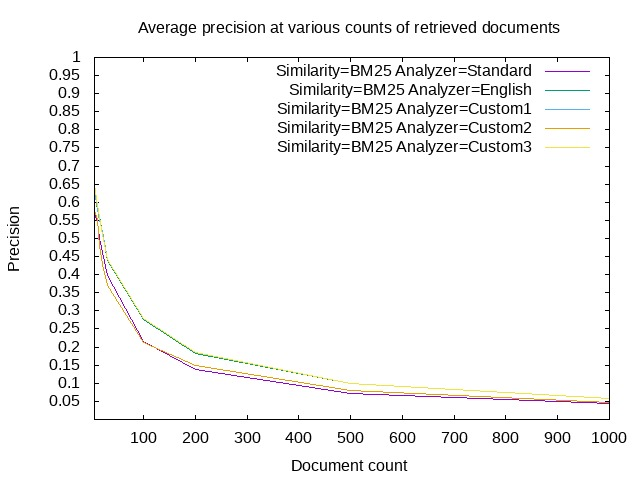
\includegraphics[width=8cm, height=6cm]{images/avg_pre_bm25.jpg}}
  \vspace*{-3mm}
  \caption{Average precision at different number of retrieved documents using BM25 Similarity}
  \label{fig:exp1}
\end{figure}
\vspace*{-4mm}
\begin{figure}[!htbp]
  \centerline{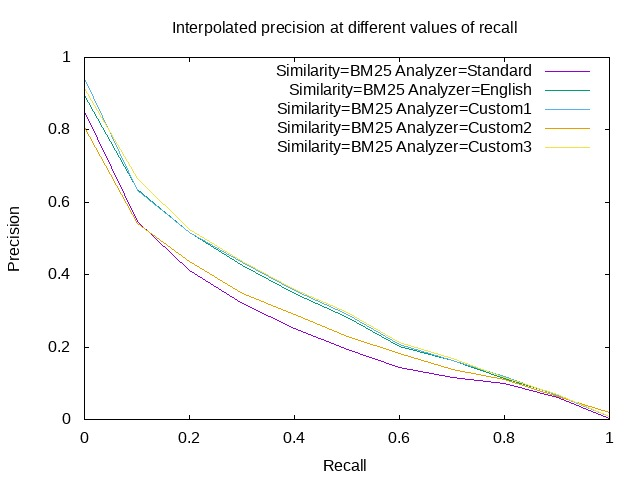
\includegraphics[width=8cm, height=6cm]{images/pr_bm25.jpg}}
  \vspace*{-3mm}
  \caption{Interpolated precision at different values of recall using BM25 Similarity}
  \label{fig:exp2}
\end{figure}
\vspace*{-4mm}
\begin{figure}[!htbp]
  \centerline{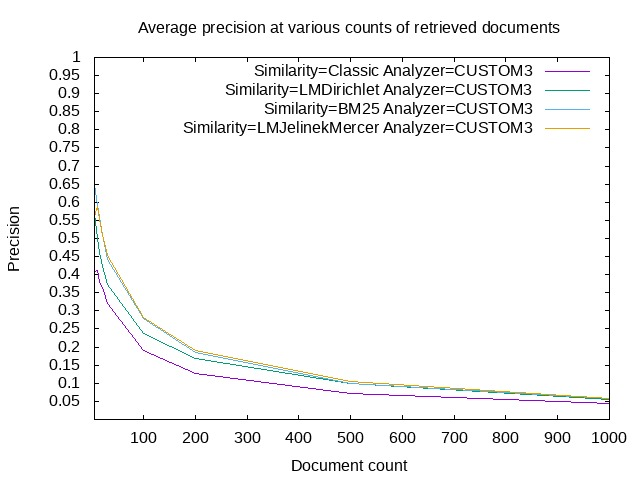
\includegraphics[width=8cm, height=6cm]{images/avg_pre_cus3.jpg}}
  \vspace*{-3mm}
  \caption{Average precision at different number of retrieved documents using CUSTOM3 analyzer with various Similarities}
  \label{fig:exp3}
\end{figure}
\vspace*{-4mm}
\begin{figure}[!htbp]
  \centering
  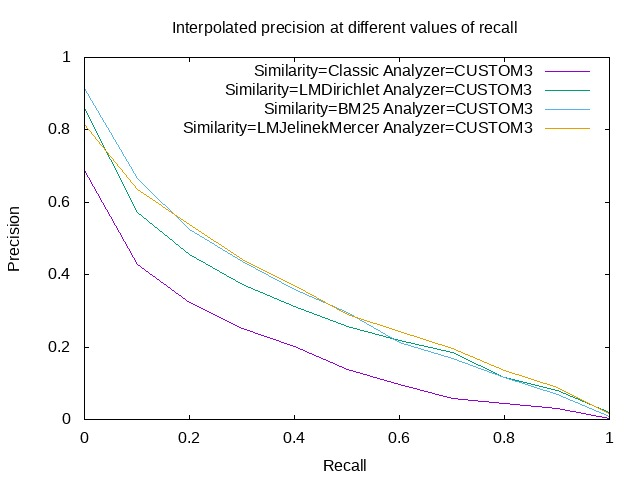
\includegraphics[width=\linewidth]{images/pr_cus3.jpg}
  \vspace*{-3mm}
  \caption{Interpolated precision at different values of recall using CUSTOM3 analyzer with various Similarities}
  \label{fig:exp4}
\end{figure}
